\documentclass{article}
\usepackage[margin=3cm]{geometry}

\usepackage{graphicx}
\usepackage{float}

\begin{document}
	
	\title{
		\line(1,0){500}\\
		[6mm]
		\bfseries Architectural Requirements Specifications and Design 
		\\
		[6mm] 
		NavUP System
		\line(1,0){500}\\
		[15mm]}
	
	\author{
		Josef Alberts - 14395283\\ 
		Gregory Austin - 14039712\\ 
		Jocelyn Bondjobo - 13232852\\ 
		Claudio Da Silva - 14205892\\ 
		Thomas Honiball - 15348751\\
		Lesego Makaleng - 15175716}
	
	\maketitle{}
	\pagebreak
	\tableofcontents
	\pagebreak

		
	\section{Introduction}
	
	The architectural requirements specification and design document, is aimed at identifying the architectural and design aspects of the system, with regards to the NavUP system in this particular instance
	
		\subsection{Purpose}
		
		The purpose of this document will be to determine the best course of action with regards to architectural design, including the requirements set forth, the constraints placed upon it and the design decisions going forward,including the architectural patterns, system design and technologies selected to solve the various requirements and constraints that have been identified.
	
		\subsection{Definitions, Acronyms, and Abbreviations}
			
			\begin{itemize}
				
				\item \textbf{GIS} \textbf{\textit{(Geographic Information System)}} \\
				\newline
				A geographic information system (or GIS) is a system designed to capture, store, manipulate, analyze, manage, and present spatial or geographic data.\\
				
				\item \textbf{GPS} \textbf{\textit{(Global Positioning System)}} \\
				\newline
				A radio navigation system that allows land, sea, and airborne users to determine their exact location, velocity, and time 24 hours a day, in all weather conditions, anywhere in the world.
			
			\end{itemize}

	\section{Requirements and Constraints}
		
		\subsection{External Interface Requirements}
		
			\subsubsection{User interfaces}
			
				\begin{figure}[H]
					
					\centering{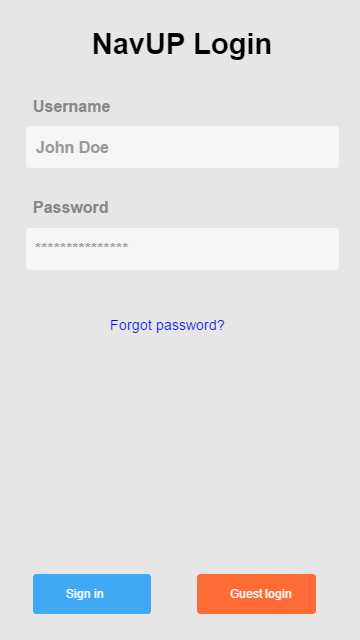
\includegraphics[width=0.25\linewidth]{./images/mocks/login_page.jpg}}
					\caption{Login Page}
					
					
				\end{figure}
			
				With regards to the login page (Figure 1), it is important to note the lack of distraction and the clear and concise labels given to each element. This ensures users of any kind have a simple straight forward means of using the application. Both sign in and guest login are provided as options, as well as a password recovery means.
			
				\begin{figure}[H]
					
					\centering{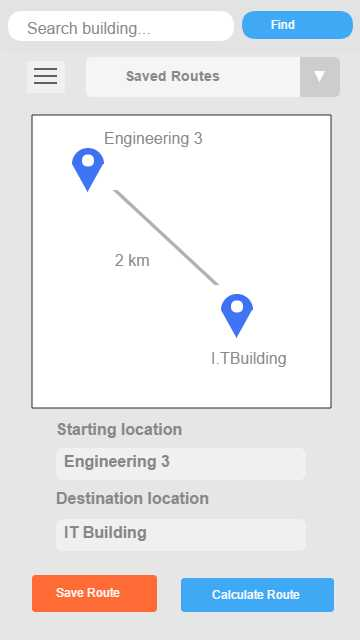
\includegraphics[width=0.25\linewidth]{./images/mocks/main_page.jpg}}
					\caption{Main Page}
				
				\end{figure}

				With regards to the main page (Figure 2), we see that all the options are presented in an easy to understand way. Elements which take up minimal room yet offer a lot such as drop-down boxes are used in order to save space and look neat, but provide the user with all the requirements in plain sight. We see a method to both calculate and select routes is available, as well as a method to search for what is required. The most important thing to note is the map being the center of attention, as it is the most important part of the application, it is made to stand out and take the focus of the user.
			
				\begin{figure}[H]
					
					\centering{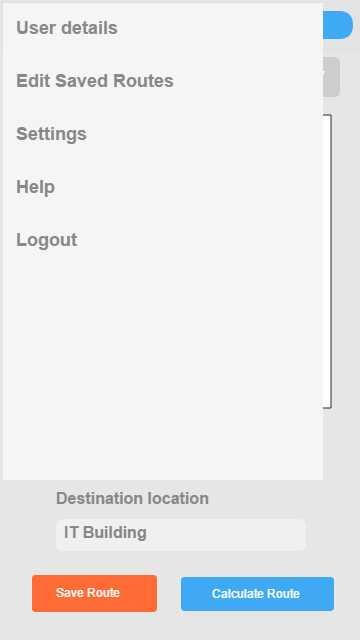
\includegraphics[width=0.25\linewidth]{./images/mocks/navigation_page.jpg}}
					\caption{Navigation Bar On Main Page}
					
				\end{figure}
			
				With regards to the navigation bar (Figure 3), we see that it is called via the hamburger button present on the main page(Figure 2) and the user page (Figure 4). This ensures that navigation is available wherever needed. Most importantly though, it ensures that the help item provided is always available when anybody is stuck, as well as the option to logout whenever needed. By keeping a consistent navigation menu, we also ensure that all pages will be the same, thus users will not be required to search hours for a button that might be in a different location or not exist on that page.
			
				\begin{figure}[H]
					
					\centering{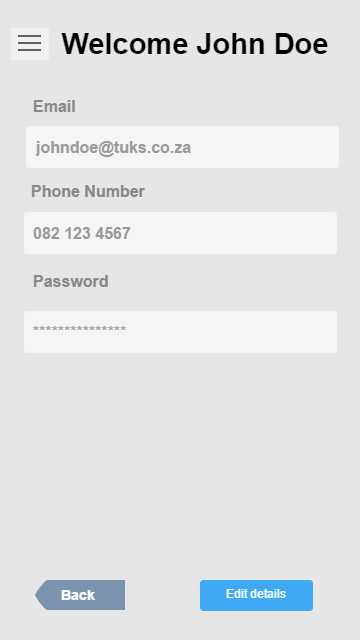
\includegraphics[width=0.25\linewidth]{./images/mocks/user_page.jpg}}
					\caption{User Details Page}
					
				\end{figure}
			
				With regards to the user details page(Figure 4), we see that a concise and easy display with clear labels is given to allow users to change the details they need, while keeping important identification factors like Usernames the same, and not giving the option to change them. We see again navigation is present, as well as an easy method of returning to the main screen. \\
				
				With regards to all the figures, a constant font and colour should be used throughout, and should preferably make accommodation for various disabilities such as colour blindness, thus not being too colorful, or visual impairment, thus not making text too small. The layout should remain consistent across resolutions and should accommodate as many different models of device as possible, from phone to tablet and more.\\
				
				While not explicitly shown, a preferably non-mobile administrator management page should be given to allow those running the server side of the system to make changes. This page would be required to be intuitive, but not necessarily appealing.
			
			\pagebreak
			
			\subsubsection{Hardware interfaces}
			
			The device types used by the system are thought to be mobile devices such as phones and tablets, as well as a physical computer on which to run the server itself.\\
			
			The system makes use of the internal hardware of the device it is on, interacting with things such as:
			
				\begin{itemize}
					\item The device's GPS, via internal means, thus natively connecting via the device's operating system in order to collect location data.
					\item The device's Internet connection, via internal means, thus natively connecting via the device's operating system in order to pull outside data.
				\end{itemize}
			
			The system however also plans to make use of some external devices, such as:
			
				\begin{itemize}
					\item Cameras, placed around the campus in order to deal with traffic detection and possibly provide heat-maps, it would communicate to the server via the internal network and the server with the device via JSON calls .
				\end{itemize}
			
			\subsubsection{Software interfaces}
			
			As stated, the system will consist of two main components, the Server and the Client.The Server is to be run off a high powered computing device, and the client side shall be run off a mobile device such as a phone or tablet. The communication method between these two modules will be that of a REST API. This means that the two components will communicate via an Internet connection, where JSON data is sent between the two components in order to transfer the required data.\\
			
			The server will connect with a database in order to store information, likely via a native connection built into the server architecture.\\
			
			The client will communicate with the internal structure of the device via native libraries, such as Android's native GPS API.
			
			\subsubsection{Communication interfaces}
			
			The software is to make use of the following communication protocols:
			
				\begin{itemize}
					\item REST, which will be the foundation of delivering data between the server and the client.
					\item Native Notifications, to allow a device to deliver information from inside the application to the recipient.
					\item Email protocols such as SMTP, to allow sending of emails for things such as verification or other updates.
					\item SMS protocols, as stated in the requirements SMS may be implemented as a notification method, and thus require an SMS server to broadcast.
				\end{itemize}
		
		\pagebreak
		
		\subsection{Performance Requirements}
		
		The NavUP system is expected to adhere to the following performance requirements:
		
			\begin{itemize}
				
				\item \textbf{Response Time}
					\begin{itemize}
						\item It is required that the response time be fast enough that the time taken to calculate the destination will not cancel out the time that it saves to use the calculated route, thus calculations should be as fast possible, estimated at under half a minute per calculation.
						\item It is expected that the time between the server and any outside device it may be using is fast enough that the data transmitted still remains current.
					\end{itemize}

			\end{itemize}
		
			\begin{itemize}
				
				\item \textbf{Intuitive Design}
				\begin{itemize}
					\item It is expected that the design of the client side is easy to use, and can be figured out by the average person without the need for any help. Furthermore it is expected that the design remain appealing in doing so.
					\item It is expected that the design for the server side is somewhat intuitive, and can be figured out with minimal effort if a new administrator is to take over. A steeper learning curve for the server may be expected than that of the client as the administrator is expected to be knowledgeable with the software.
				\end{itemize}
				
			\end{itemize}
		
			\begin{itemize}
	
				\item \textbf{Reliability}
				\begin{itemize}
					\item It is expected that the data transferred from the server to the client is indeed accurate up to a degree of fault to be determined.
					\item It is expected that the data held by the server is protected in case of a fault that may occur by methods such as backups.
					\item It is expected that the system is protected against downtime in the case of a hardware failure on the server end.
				\end{itemize}	
	
			\end{itemize}
		
			\begin{itemize}
			
				\item \textbf{Security}
			
				\begin{itemize}
					\item It is expected that the transfer of location data is kept anonymous as far as possible so that personal location and travel routes are kept private.
					\item It is expected that the transfer of a users detail is encrypted in a way that nobody except the user has access to important items such as email and password.
					\item It is expected that access to the server and its details is restricted solely to those with proper access, via secure passwords and possibly additional authentication methods.
				\end{itemize}	
			
			\end{itemize}				
		
		\pagebreak
		
		\subsection{Design Constraints}
		
			\begin{itemize}
				
				\item \textbf{Client Constraints}
				
				\begin{itemize}
					\item The client should be able to run using the power of an average mobile phone, thus should adhere to a RAM limit of around 200mb maximum.
					\item The client should be able to fit on an average mobile phone, thus an application should take up minimal space, around 100mb maximum.
				\end{itemize}	
				
			\end{itemize}
		
			\begin{itemize}
				
				\item \textbf{Server Constraints}
				
				\begin{itemize}
					\item The server should be able to run using the power of a server specified computer, and not that of a server farm, thus should adhere to a RAM limit of around 4GB if possible, with around an 8GB maximum
					\item The server should fit on a regular PC, thus the application size, along with the size of the database, should be small enough to fit on a standard server sized hard drive, to a maximum of 2TB if possible.
				\end{itemize}	
				
			\end{itemize}
		
			\begin{itemize}
				
				\item \textbf{Data constraints}
				
				\begin{itemize}
					\item It is expected that data charges should occur, but in the event one has minimal access to campus WIFI, JSON packets transfered should remain as small and infrequent as possible to maintain a decent level of quality when off said unlimited connection.
					\item Data kept should remain minimal as space for data will too be minimal. As the University shall not be capable of a data farm for such an application, the data stored should only be that used in important frequent calculations and that of users due to database constraints. 
				\end{itemize}	
				
			\end{itemize}
		
			\begin{itemize}
				
				\item \textbf{Flexibility constraints}
				
				\begin{itemize}
					\item At no point in time should the software be locked in to a specific system or coupled tightly enough the the campus that the ability to move this system and change its use becomes absolutely impossible.
				\end{itemize}	
				
			\end{itemize}				
		
		\pagebreak
		
		\subsection{Software System Attributes}
				The following software attributes can be classified as run-time qualities :
		\begin{itemize}
			\item \textbf {Performance}
			\begin{enumerate}
				\item \textbf{Description} \\
				Application performance can be defined as the amount of work that can be accomplished by an application in question in a measured time interval. The time interval is normally measured in seconds, where the amount of work can be defined as the throughput, latency or data transmission time.
				\begin{itemize}
					\item \textbf{Throughput} \\
					The number of requests and responses which can be processed by the system in a given time interval for example the time the application takes to locate its user on the map using wifi access points and gps.
					\item \textbf{Latency and Data transmission time} \\
					A time interval measured as the time it takes to service a request such as to find the best route or path to guide the user to a certain destination. 
				\end{itemize}
	
				The aim for this system, is to increase the throughput and decrease the latency. As the developer has no control over the network medium used, s/he must aim for a minimal request and response payload as to decrease the data transmission time.
				\item \textbf{Justification} \\
				Our aim for this system is to increase throughput, decrease latency and data transmission time. This will ensure we have a system that is responsive at all times, including peak times and delivers an excellent user experience.
				\item \textbf{Requirements}
				\begin{itemize}
					\item Function calls must be timed and benchmarked and this data should be logged.
					\item Network responses should be cached on server side to lighten the load on the device.
				\end{itemize}
			\end{enumerate}
			\item \textbf {Reliability}
			\begin{enumerate}
				\item \textbf{Description} \\
				The designed system needs to be accessible from both inside and outside buildinds at the University of Pretoria campuses as well as from other networks, especially on other campuses. The system should be reliable in its accessibility.
				\item \textbf{Justification} \\ 
				The system must not be unreliable in that it crashes under large workloads for example when many users are actually using the application and some users get denied service during work critical times when workloads are high. This causes a detriment in user productivity. To ensure that the system can be used confidently as a tool to increase productivity and ease the work process, the development aim must be for the system to be as reliable and accessible as possible.
				\item \textbf{Requirements}
				\begin{itemize}
					\item To enable access of data from the Android or IOS app even when offline such as preferences, events, etc..
				\end{itemize}
			\end{enumerate}
			\item \textbf {Scalability}
			\begin{enumerate}
				\item \textbf{Description} \\
				Scalability refers to the application in question's ability to handle an above normal workload for example when many users are currently using the app as it must provide and visualise information related to pedestrian traffic on campus for example in the form of heat maps of user locations.
				\item \textbf{Justification} \\
				The system needs Scalability because it needs to support many users at the same time.
				\item \textbf{Requirements}
				\begin{itemize}
					\item The system should be able to handle the growing amount of data or number of users using the app at the same time.
				\end{itemize}
			\end{enumerate}
		\item \textbf {Security}
		\begin{enumerate}
			\item \textbf{Description} \\
			Security in application software refers to authentication, authorization, data security and accounting. Authentication refers to the systems' ability to provide a way of identifying a user, normally with our system it will identify its users from the device name.
			\item \textbf{Justification} \\
			Security is a important aspect of any software product. In terms of information security, we are concerned about integrity, availability, confidentiality and non-repudiation in that order. 

			\item \textbf{Requirements}
			\begin{itemize}
				\item System should be resistant hacking as some people could use it to steal some personal information on the device about the user.
			\end{itemize}
		\end{enumerate}
	\end{itemize}
	
	\pagebreak
	
	\section{Module Design}
	
		\subsection{GIS Subsystem}
		
			\begin{figure}[H]
				
				\centering{\includegraphics[width=\textwidth, height=!]{./images/class/GISClassDiagram.png}}
				\caption{Class diagram for the GIS module}
				
			\end{figure}
			
			\begin{figure}[H]
				
				\centering{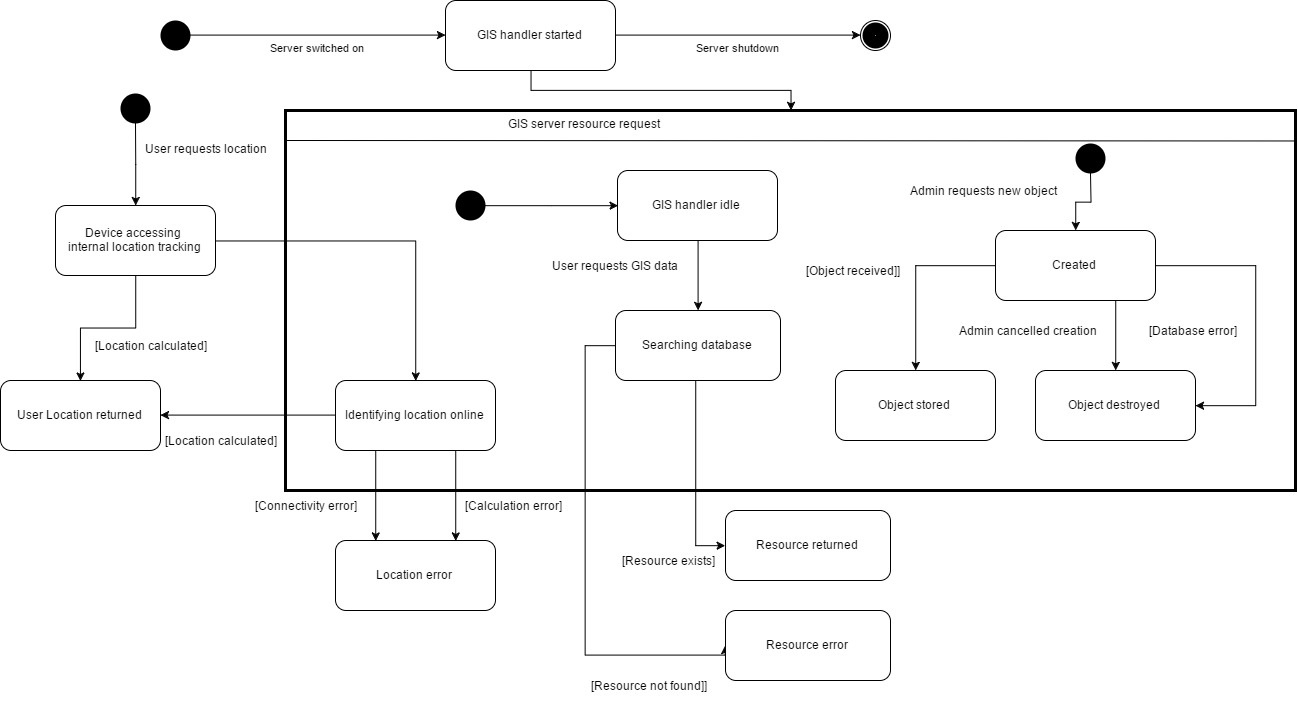
\includegraphics[width=\textwidth, height=!]{./images/state/gis_state.jpg}}
				\caption{State diagram for the GIS module}
				
			\end{figure}

		\subsection{Notification Subsystem}
			
			\begin{figure}[H]
				
				\centering{\includegraphics[width=\textwidth, height=!]{./images/class/NotificationsClassDiagram.png}}
				\caption{Class diagram for the Notification module}
				
			\end{figure}
			
			\begin{figure}[H]
			
				\centering{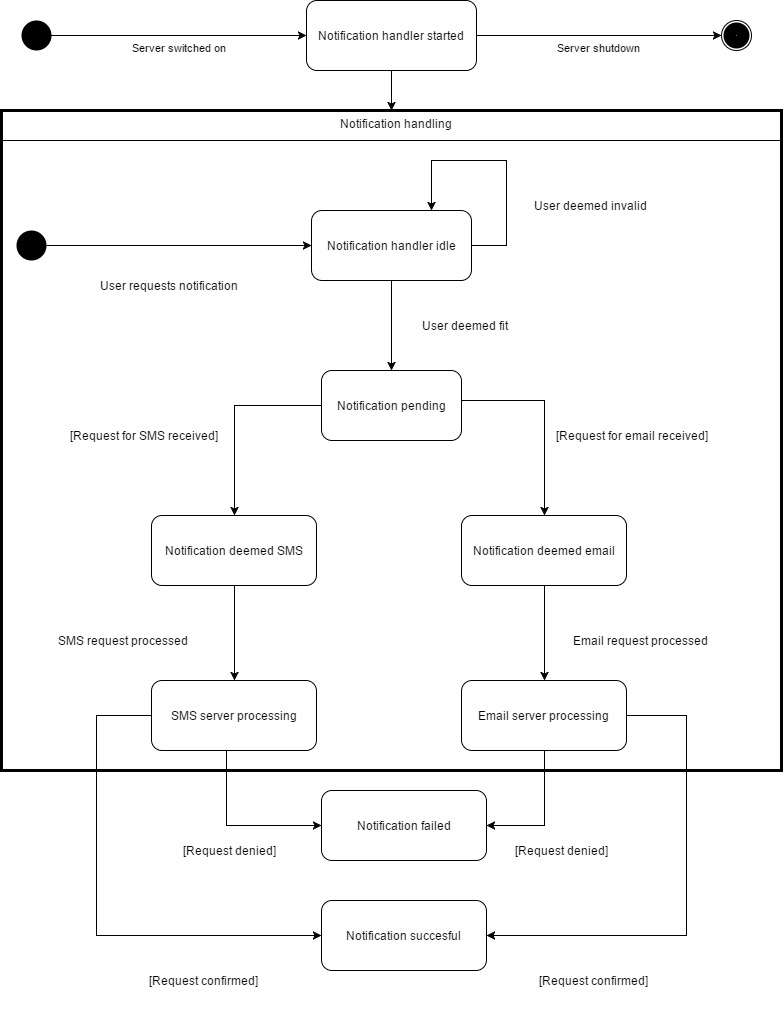
\includegraphics[width=\textwidth, height=!]{./images/state/notifications_state.jpg}}
				\caption{State diagram for the Notifications module}
			
			\end{figure}
	
		\subsection{Navigation Subsystem}
		
			\begin{figure}[H]
				
				\centering{\includegraphics[width=\textwidth, height=!]{./images/class/NavigationClassDiagram.png}}
				\caption{Class diagram for the Navigation module}
				
			\end{figure}		
			
			\begin{figure}[H]
				
				\centering{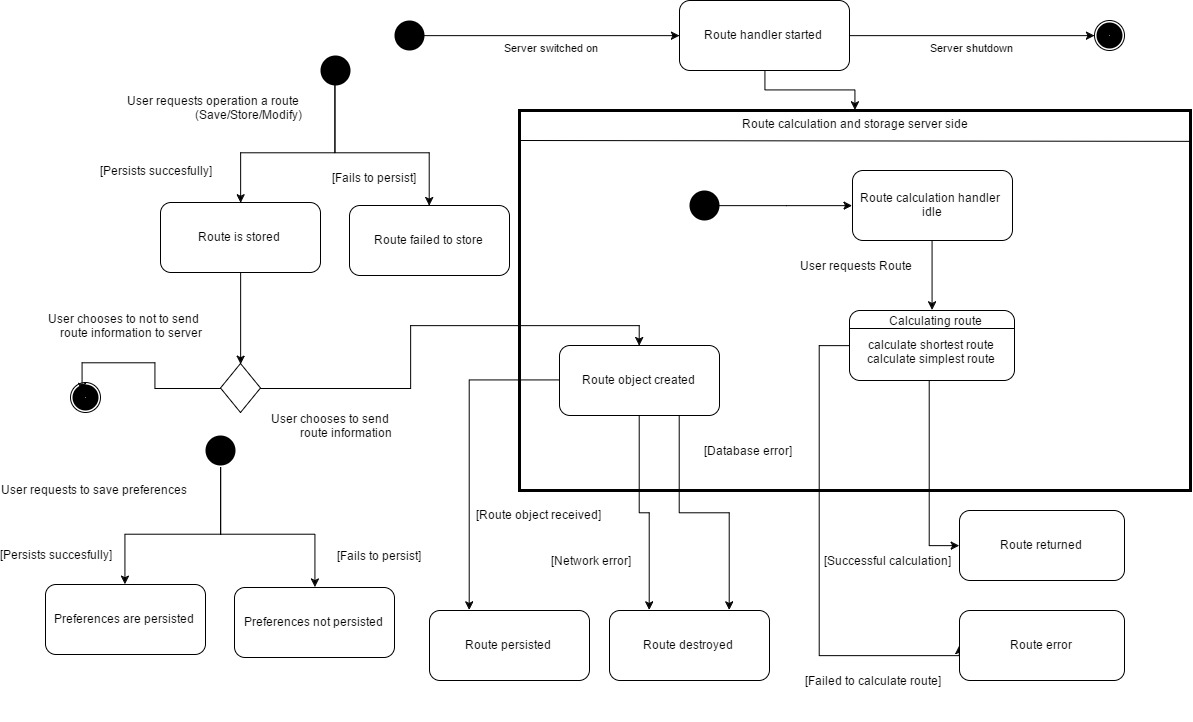
\includegraphics[width=\textwidth, height=!]{./images/state/navigation_state.jpg}}
				\caption{State diagram for the Navigation module}
				
			\end{figure}
	
		\subsection{Events Subsystem}
		
			\begin{figure}[H]
				
				\centering{\includegraphics[width=\textwidth, height=!]{./images/class/EventsClassDiagram.png}}
				\caption{Class diagram for the Events module}
				
			\end{figure}
		
			\begin{figure}[H]
				
				\centering{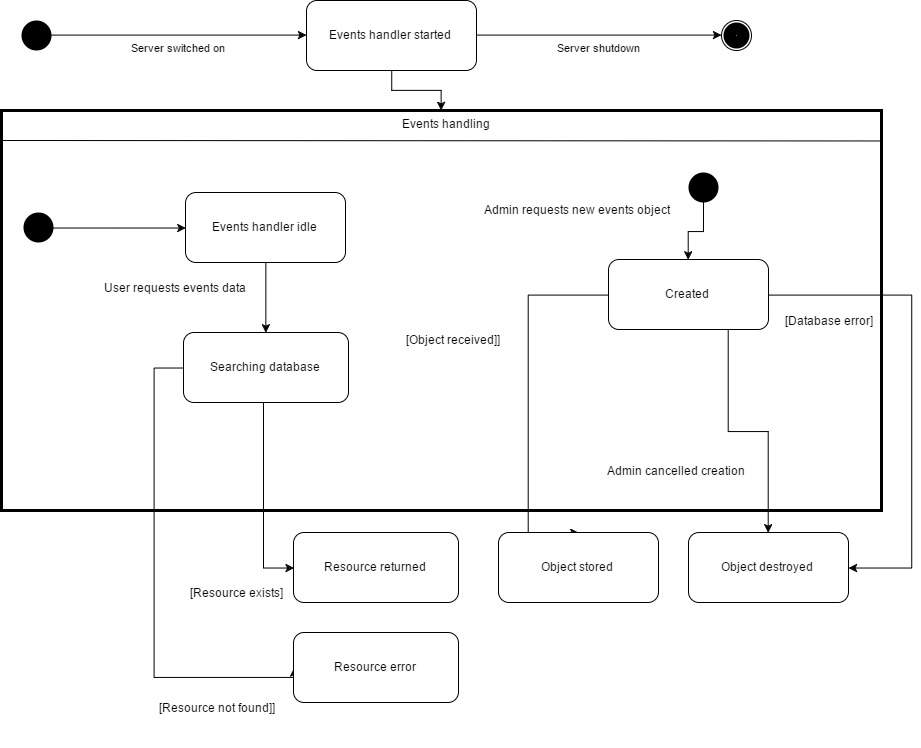
\includegraphics[width=\textwidth, height=!]{./images/state/events_state.jpg}}
				\caption{State diagram for the Events module}
				
			\end{figure}
			
		\subsubsection{Create Event}
			\begin{figure}[H]
				\centering{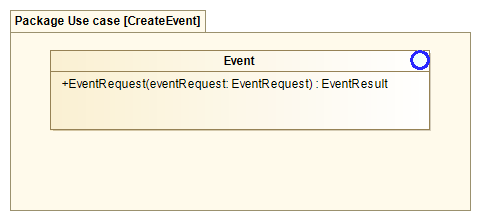
\includegraphics[width=\textwidth, height=!]{./Use Cases/package createEvent.png}}
				\centering{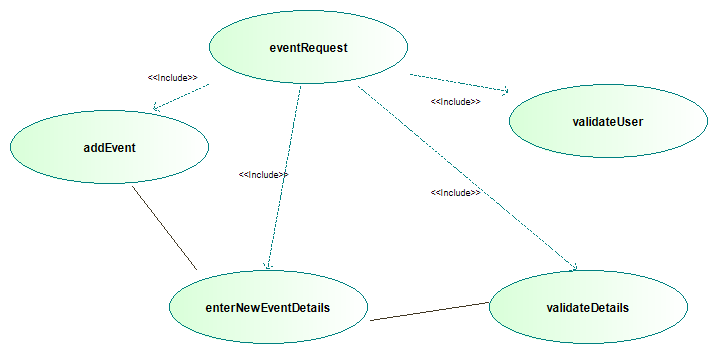
\includegraphics[width=\textwidth, height=!]{./Use Cases/createEvent.png}}
				\caption{Use cases for Create Event}
			\end{figure}
	
	\pagebreak
	
	\section{System assessment}	
	
		\subsection{Technology choices}
		
		\subsubsection{Android client}
		
			\begin{enumerate}
				 \item \textbf{Programming Languages}
				\begin{itemize}
					\item Java
					\item eXtensible Markup Language (XML)
				\end{itemize}
			\item \textbf{Frameworks}
				\begin{itemize}
					\item Android Studio
				\end{itemize}
			\item \textbf{Libraries}
				\begin{itemize}
					\item Android Butterknife
				\end{itemize}
			\item \textbf{Database System} \\ \\ 
			Couchbase Mobile which consists of:
				\begin{itemize}
	 				\item Couchbase Lite
					\item Couchbase Sync Gateway
					\item Couchbase Server
				\end{itemize}
				\item \textbf{Operating System}
			\begin{itemize}
	 				\item Android 4.0. Devices and upwards
				\end{itemize}
			\item \textbf{Dependency Management and Build Tools}
				\begin{itemize}
					\item Gradle
				\end{itemize}
			\end{enumerate}
	
		\subsubsection{IOS client}
		
			\begin{enumerate}
			 \item \textbf{Programming Languages}
				\begin{itemize}
					\item Objective C
				\end{itemize}
			\item \textbf{Frameworks}
				\begin{itemize}
					\item Apple's Swift
				\end{itemize}
			\item \textbf{Libraries}
				\begin{itemize}
					\item CocoaPods
					\item Carthage
				\end{itemize}
			\item \textbf{Database System}
				\begin{itemize}
	 				\item AFNetworking
					\item JSONModel
					\item MagicalRecord
					\item SDWebImage
					\item ReactiveCocoa
				\end{itemize}
			\item \textbf{Operating System}
				\begin{itemize}
	 				\item IOS devices
				\end{itemize}
			\item \textbf{Dependency Management and Build Tools}
				\begin{itemize}
					\item Swift Package Manager (SPM)
				\end{itemize}
			\end{enumerate}
	
		\subsubsection{Server side}
		
				\begin{enumerate}
				\item \textbf{Programming Languages}
				\begin{itemize}
					\item HMTL 5
					\item CSS 3
					\item Javascript
					\item jQuery
				\end{itemize}
				\item \textbf{Frameworks}
				\begin{itemize}
					\item N/A
				\end{itemize}
				\item \textbf{Libraries}
				\begin{itemize}
					\item Bootstrap as library for CSS
				\end{itemize}
				\item \textbf{Database System}
				\begin{itemize}
					\item mySQL
				\end{itemize}
				\item \textbf{Operating System}
				\begin{itemize}
					\item Linux (Preferably)
					\item Windows
					\item MacOS (Possibly)
				\end{itemize}
				\item \textbf{Dependency Management and Build Tools}
				\begin{itemize}
					\item N/A
				\end{itemize}
			\end{enumerate}
		
			
\end{document}
